\documentclass[../main.tex]{subfiles}

\begin{document}

The last piece of a puzzle is to invoke creation of the Adjuster. This is done by the Adjust endpoint handler, which asynchronously starts the creation using \textit{OpenShiftAdjusterPodController}\footnote{\url{https://github.com/project-ncl/reqour/blob/akridl-thesis/rest/src/main/java/org/jboss/pnc/reqour/rest/openshift/OpenShiftAdjusterPodController.java}}  and immediately afterwards returns 202 Accepted.

\textit{OpenShiftAdjusterPodController} uses OpenShift API from Quarkus\footnote{\url{https://quarkus.io/guides/kubernetes-client##openshift-client}}. Concrete details of the deployment are injected during runtime. Adjuster deployment hierarchy is shown in Figure \ref{fig:adjuster-deployment}.

\begin{figure}
  \begin{center}
    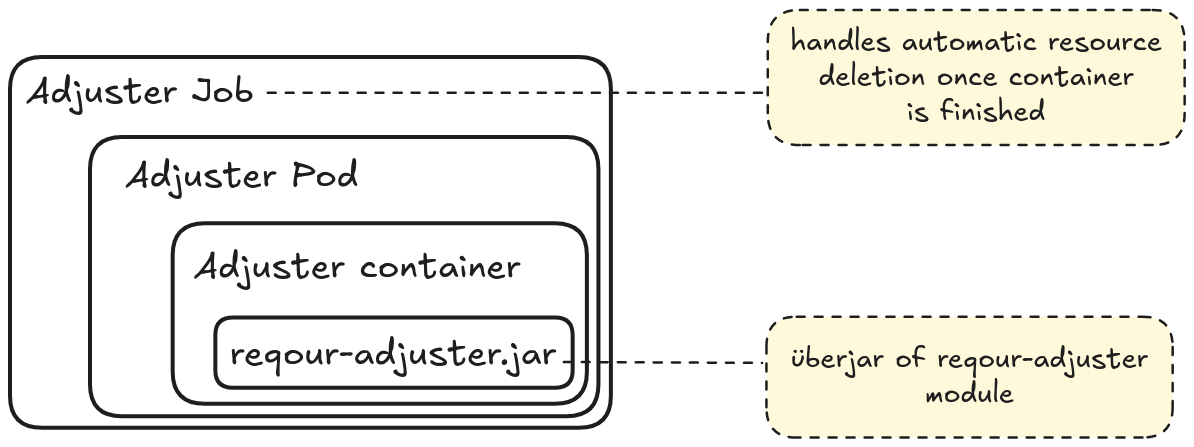
\includegraphics[width=\textwidth]{images/adjuster-deployment.png}
  \end{center}
  \caption{Hierarchy of Adjuster deployment}
  \label{fig:adjuster-deployment}
\end{figure}

\end{document}
